\documentclass[russian,a4paper,12pt]{scrartcl}
\usepackage{babel}
\usepackage[utf8]{inputenc}
\usepackage[left=3cm,right=1cm,top=1cm,bottom=1cm]{geometry}
\usepackage{misccorr}
\usepackage{amsmath}
\usepackage{minted}
\usepackage{graphicx}
\usepackage{xcolor}

\begin{document}
	\begin{center}
	
		\vspace{10mm}
		{ГУАП}\par \vspace{0.5cm}
		{КАФЕДРА №14} \par 
		
	\vspace{20mm}
	\begin{flushleft}
		{ОТЧЕТ}\par
		{ЗАЩИЩЕН С ОЦЕНКОЙ}\par \vspace{2mm}
		{ПРЕПОДАВАТЕЛЬ}\par
		\[
		\underset{\text{должность}}{\underline{\hspace{0.5cm}\text{\strut доц.,к.т.н.}\hspace{0.5cm}}}
		\quad\underset{\text{подпись, дата}}{\underline{\strut \hspace{4cm}}}
		\quad\underset{\text{инициалы, фамилия}}{\underline{\hspace{1cm}\text{\strut К.А. Курицин}\hspace{1cm}}}
		\]
	\end{flushleft}
	\vspace{20mm}

		 \text{ОТЧЕТ ПО ЛАБОРАТОРНОЙ РАБОТЕ №2}\par
		 \vspace{15mm}
		 \text{по курсу: ТЕХНОЛОГИЯ ПРОГРАММИРОВАНИЯ} \par
		
	\vspace{40mm}

	\begin{flushleft}
		\text{РАБОТУ ВЫПОЛНИЛИ}\vspace{2mm}
		$
		\text{CТУДЕНТЫ ГРУППЫ}\quad 
		\underline{\strut 1441} 
		\quad\underset{\text{подпись, дата}}{\underline{\strut \hspace{3cm}}}\quad
		\underset{\text{инициалы, фамилия}}{\underline{\text{\strut М.А. Конаков, А.В. Рещенко}}}
		$
	\end{flushleft}

	\vspace{50mm}
	
		\text{Санкт-Петербург 2016}
	\newpage
	
	\end{center}
	\begin{flushleft}
	\section{Постановка задачи}
		Реализовать класс синхронизации семафор.
		Класс инкапсулирует работу объекта синхронизации, который содержит счетчик между нулем и заданным максимальным значением. Значение счетчика увеличивается каждый раз, когда поток завершает ожидание освобождения семафора, и уменьшается, когда поток освобождает семафор. В случае, если значение счетчика достигает максимального значения, потоки ожидают освобождение семафора.
		Если указано максимальное значение счетчика, равное 1, то семафор функционально должен вести себя как критическая секция (critical section).
	\end{flushleft}
	\section{Листинги}
	\usemintedstyle{autumn}
	\inputminted[
			frame=lines,
			framesep=2mm,
			baselinestretch=1.2,
			fontsize=\footnotesize,
			linenos
			]{cpp}{main.cpp}
	\newpage
	\section{Примеры работы программы}
	\begin{center}
		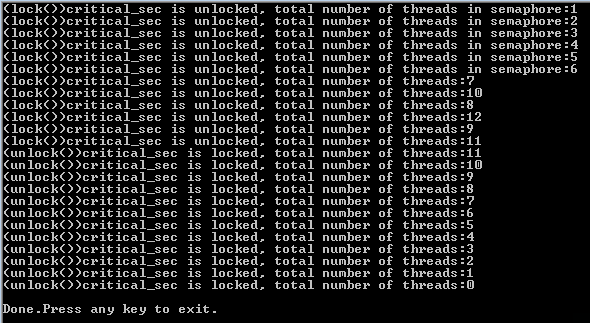
\includegraphics[scale=0.7]{Screen}\\
		\text{Семафоров 6, потоков 12}\\
	\end{center}
\end{document}
